\section{Basic Notation and Concepts} \label{sec:notation}
% \alessio{As of now this is a stash of general stuff that is important to explain in a general section.}

%\par\noindent\rule{\textwidth}{0.4pt}

\begin{definition}[String]\label{def:string}
    A \textbf{string} is a sequence of characters $S = s_1s_2\ldots s_n$ drawn from an alphabet $\Sigma$.
\end{definition}
We use $|S| = n$ to denote the length of $S$.
The set of all strings is represented as $\Sigma^*$, which also contains the empty string $\varepsilon$.\newline
The notation $S[i] = s_i$ denotes the $i$-th character of $S$, and $S[i\dots j]$ the substring $s_is_{i+1}\ldots s_j$, for $1 \leq i,j \leq n$.
Therefore, a prefix of $S$ is a substring of the type $S[1\dots j]$, while a suffix is a substring $S[i \dots n]$.

\begin{definition}[Subsequence]
    $S' = s'_1\ldots s'_m$ is a \textbf{subsequence} of some string $S = s_1\ldots s_n$ if there exist a strictly increasing sequence of indices $1 \le i_1 < i_2 < \ldots < i_m \le n$ such that $s'_j = s_{i_j}$ for all $j = 1,\ldots, m$.    
\end{definition}
In other words, a subsequence is a sequence of characters from a string that are not necessarily contiguous, but are in the same order as they appear in the original string.

We recall the following important notation for strings from the introduction section: 
\vspace{-1em}
\setsubseqdef*

%\par\noindent\rule{\textwidth}{0.4pt}
A basic understanding of formal grammars is crucial for comprehending some of the state-of-the-art tree compression methods discussed in this thesis.
\begin{definition}[Grammar]
    A \textbf{formal grammar} is a set of rules for generating strings in a formal language. A grammar is typically defined as a 4-tuple $G = (N, \Sigma, P, S)$, where:
    \begin{itemize}
        \item $N$ is a finite set of non-terminal symbols.
        \item $\Sigma$ is a finite set of terminal symbols, disjoint from $N$.
        \item $P$ is a finite set of production rules, each of the form $(\alpha \rightarrow \beta)$, where $\alpha$ is a string of symbols from $(N \cup \Sigma)^*$ containing at least one non-terminal symbol, and $\beta$ is a string in $(N \cup \Sigma)^*$.
        \item $S \in N$ is the start symbol.
    \end{itemize}
\end{definition}

\begin{example}
    For example, consider the grammar $G = (\{S\}, \{a, b\}, P, S)$ with the following production rules in $P$:
    \begin{enumerate}
        \item $S \rightarrow aSb$
        \item $S \rightarrow \epsilon$
    \end{enumerate}
    This grammar generates the language $\{a^n b^n \mid n \geq 0\}$, which includes strings like $\epsilon$ (the empty string), $ab$, $aabb$, $aaabbb$, and so on.
\end{example}

Let us now move to the definition of rooted tree.
\begin{definition}[Tree] \label{def:rooted_tree}
    A \textbf{rooted tree} is a triple $T = (V, E, r)$ where:
    \begin{itemize}
        \item $V$ is a finite set of vertices (or nodes),
        \item $E\subseteq V \times V$ is a set of edges such that $|E| = |V|-1$ and the underlying graph is connected and acyclic,
        \item $r\in V$ is the root vertex.
    \end{itemize}
\end{definition}

We denote by $t = |V|$ the number of vertices in the tree.

\begin{definition}[Tree Terminology] \label{def:tree_terminology}
Given a rooted tree $T = (V, E, r)$, we define the following concepts:
\begin{itemize}
    \item \textbf{Parent:} For any two distinct nodes $u,v\in V$, with $v\neq r$, we say that $u$ is the parent of $v$ iff $(u, v) \in E$ and $u$ lies on the unique path from $r$ to $v$. It follows that each node $v$ (except from the root) has exactly one parent, which we denote as $\textup{parent}(v)$. 
    \item \textbf{Children:} For a vertex $u\in V$, we define the set $\textup{children}(u) = \{v \in V | (u,v)\in E \land u = \textup{parent}(v)\}$
    \item \textbf{Leaves:} A vertex $v \in V$ is a \textit{leaf} if it has no children, i.e., there is no edge $(v, w) \in E$ for any $w \in V$.
    \item \textbf{Degree:} The \textit{degree} of a node $u$, denoted $\text{deg}(u)$, is its number of children.
    \item \textbf{Depth:} The \textit{depth} (or level) of a vertex $v$, denoted $\text{depth}(v)$, is the length of the unique path from the root $r$ to $v$ minus 1. The root has depth 0.
    \item \textbf{Height:} The \textit{height} of the tree is the maximum depth among all its leaves.
    \item \textbf{Subtree:} For any vertex $v \in V$, the \textit{subtree rooted at $v$} is the tree $T_v = (V', E', v)$ where $V'$ contains $v$ and all its descendants, and $E'$ contains all edges between vertices in $V'$.
    \item \textbf{Linearization:} A \textit{linearization} of a tree is a total ordering of its vertices that respects some traversal order (e.g., pre-order, post-order, or in-order).
\end{itemize}
\end{definition}

% \par\noindent\rule{\textwidth}{0.4pt}

\section{Finite State Automata} \label{sed:fsa}
Finite automata are fundamental computational models that recognize regular languages through a finite set of states and transitions. They provide an elegant mathematical framework for representing and manipulating collections of strings, making them particularly suitable for applications in pattern matching, lexical analysis, and data compression. In the context of this thesis, finite automata serve as the underlying representation for tries and other string data structures, enabling efficient compression through state minimization.

Let $L \subseteq \Sigma^*$ be a finite set of strings. $L$ can be represented in many different ways, such as enumeration, context-free grammars, regular expressions, or automata.

\begin{definition}[Non-deterministic Finite Automaton] \label{def:nfa}
    A \textbf{non-deterministic finite automaton} (NFA) is a 5-tuple $\nfa = (Q, \Sigma, \delta, q_0, F)$ where:
    \begin{itemize}
        \item $Q$ is a finite set of states,
        \item $\Sigma$ is a finite alphabet,
        \item $\delta: Q \times \Sigma \to \mathcal{P}(Q)$ is the transition function, where $\mathcal{P}(Q) = \{A | A \subseteq Q \}$ is the powerset of $Q$,
        \item $q_0 \in Q$ is the initial state,
        \item $F \subseteq Q$ is the set of final (accepting) states.
    \end{itemize}
\end{definition}

An NFA processes an input string $S \in \Sigma^*$ one symbol at a time, starting from $q_0$ and following the transitions specified by $\delta$.
Let $\hat\delta: Q \times \Sigma^* \to \mathcal{P}(Q)$ be the extension of $\delta$ to strings defined as follows.
For all $u \in Q$, $a \in \Sigma$, and $\alpha \in \Sigma*$:
\[
\hat\delta(u,\varepsilon)=\{u\}, \qquad
\hat\delta(u,\alpha a)=\bigcup_{v \in \hat\delta(u,\alpha)} \delta(v,a).
\]
Therefore, $\delta(q_0,\alpha)$ denotes the set of states that can be reached from the start state $q_0$ by reading $\alpha$.
A string $S$ is \emph{accepted} if $\delta(q_0, S)\cap F \neq \emptyset$, or, in other words, if the automaton ends in any state $q \in F$ after processing the entire string.
The set of all strings accepted by $\nfa$ is called the \emph{language} of the automaton, and is denoted as
\[
\lang{\nfa}=\{S \in \Sigma^* \mid \delta(q_0, S)\cap F \neq \emptyset\}.
\]

Deterministic Finite Automata are a special case of NFAs, where each state has exactly one outgoing transition per character, i.e., $|\delta(q, a)| = 1$.

\begin{definition}[Deterministic Finite Automaton] \label{def:dfa}
    A \textbf{deterministic finite automaton} (DFA) is a 5-tuple $\dfa = (Q, \Sigma, \delta, q_0, F)$ where:
    \begin{itemize}
        \item $Q$ is a finite set of states,
        \item $\Sigma$ is a finite input alphabet,
        \item $\delta: Q \times \Sigma \rightarrow Q$ is the transition function,
        \item $q_0 \in Q$ is the initial state,
        \item $F \subseteq Q$ is the set of final (accepting) states.
    \end{itemize}
\end{definition}
Notice how the only difference between \cref{def:nfa} and \cref{def:dfa} is the return value of the transition function.
As a consequence, the expansion of $\delta$ to strings can be simplified to 
\[
    \hat\delta(u, \alpha a) = \delta(\hat\delta(\alpha), a)
\]
Similarly to NFAs, the language of a DFA is the set of strings that end at a state $q \in F$ after being processed:
\[
    \lang{\dfa} = \{S \in \Sigma^* \mid \hat\delta(q_0, a) \in F\}
\]

Also, we introduce the following notation for automata: For \( q \in Q \) we write \( I_q \) to denote the set of strings reaching \( q \) from the initial state:
\[
I_q = \{ \alpha \in \Sigma^* \mid q = \delta(q_0, \alpha) \}
\]

NFAs can be more compact in terms of the number of states required to represent a language: a well-known fact is that the smallest DFA for a language could be exponentially larger than the smallest equivalent NFA. In this thesis this will not be a concern, since we will assume that the input language is presented via a DFA (more specifically, a trie). 

%DFAs also present advantages in terms of compressibility \nicola{questa frase è in contrasto con il precedente paragrafo: spiega meglio}. For instance, as shown in \cref{thm:indexing}, when using compression schemes based on $p$-sortable automata (\cref{def:p-sorable-automaton}), DFAs offer a space advantage. A $p$-sortable DFA requires $\log p$ fewer bits per edge than its NFA counterpart, making it more space-efficient in this context. \nicola{riformula: DFA log p, mentre NFA 2log p (così non è chiaro quanto spazio occupano gli NFA)}

Finally, automata are naturally represented as labeled directed graphs, where the vertices are the states and the edges represent the transitions, labeled with characters from the alphabet.

\begin{example}
Figure \ref{fig:nfa_dfa_example} shows an example of an NFA and an equivalent DFA that both accept the language of strings over alphabet $\{a, b\}$ ending with the character `a'.

\begin{figure}[H]
    \centering
    \begin{subfigure}[b]{0.45\textwidth}
        \centering
        \begin{tikzpicture}[shorten >=1pt,node distance=2cm,on grid,auto] 
           \node[state,initial,initial text=] (q_0)   {$n_0$}; 
           \node[state,accepting](q_1) [right=of q_0] {$n_1$}; 
            \path[->] 
            (q_0) edge [loop above] node {$a,b$} ()
                  edge node {$a$} (q_1);
        \end{tikzpicture}
        \caption{}
        \label{fig:nfa_example}
    \end{subfigure}
    \hfill
    \begin{subfigure}[b]{0.45\textwidth}
        \centering
        \begin{tikzpicture}[shorten >=1pt,node distance=2cm,on grid,auto] 
           \node[state,initial, initial text=] (A) {$d_0$};
           \node[state,accepting](B) [right=of A] {$d_1$};
            \path[->] 
            (A) edge [loop above] node {b} ()
                edge node {a} (B)
            (B) edge [loop above] node {a} ()
                edge [bend right] node [above] {b} (A);
        \end{tikzpicture}
        \caption{}
        \label{fig:dfa_example}
    \end{subfigure}
    \caption{(a) An NFA and (b) an equivalent DFA for the language $(a|b)^*a$.}
    \label{fig:nfa_dfa_example}
\end{figure}
\end{example}

\subsection{Minimization} \label{sec:hopcroft}
The process of automata minimization consists of reducing the number of states in an automaton while preserving its accepted language. 
As extensively shown in the literature, determinism makes this problem much easier: while minimizing DFAs can be achieved in polynomial time, minimizing NFAs is a PSPACE--complete problem. 

Tries are inherently deterministic, since from any node, there is at most one outgoing edge for each symbol in the alphabet. 
This deterministic nature will be crucial in this work to apply powerful automata minimization techniques to compress the tree structure.

The minimization of DFAs is a well-studied problem in automata theory, and there are several algorithms available for this purpose. One of the most popular algorithms for DFA minimization is Hopcroft's algorithm, which was proposed by John Hopcroft in 1971~\cite{HOPCROFT1971189}. Hopcroft's algorithm is an efficient and simple algorithm that can minimize a DFA in $O(n \log n)$ time, where $n$ is the number of states in the DFA.

The algorithm enables computing equivalence classes of nodes, in particular, the Myhill--Nerode equivalence classes~\cite{nerode1958linear, myhill1957finite}. The Myhill--Nerode theorem states that a language is regular if and only if it has a finite number of Myhill--Nerode equivalence classes. This theorem provides a powerful tool for determining the regularity of languages and is a cornerstone of automata theory. Let us formalize the concept of equivalence classes and the Myhill--Nerode theorem.

\begin{definition}[Myhill--Nerode Equivalence Relation]
    For a language $L \subseteq \Sigma^*$ and any strings $x,y \in \Sigma^*$, we say $x$ is equivalent to $y$ with respect to $L$ (written as $x \approx_L y$) if and only if for all strings $z \in \Sigma^*$:
    \[ xz \in L \Leftrightarrow yz \in L \]
\end{definition}
That is, strings $x$ and $y$ are equivalent if they have the same behavior with respect to the language $L$: either they both lead to acceptance or both lead to rejection when any suffix $z$ is appended.

\begin{theorem}[Myhill--Nerode theorem~\cite{nerode1958linear,myhill1957finite}] \label{def:myhill-nerode}
    Let $L$ be a language over an alphabet $\Sigma$. Then $L$ is regular if and only if there exists a finite number of Myhill--Nerode equivalence classes for $L$. Specifically, the number of equivalence classes is equal to the number of states in the minimal DFA recognizing $L$.
\end{theorem}

Throughout this section let $M = (Q, \Sigma, \delta, q_0, F)$ be a DFA. For $q \in Q$ and $a \in \Sigma$, we adopt the shorthand $q.a := \delta(q,a)$. We extend $\delta$ to words by the usual recursion:
\[
\delta^{*}(q,\varepsilon) = q, \qquad
\delta^{*}(q,wa) = \delta\bigl(\delta^{*}(q,w),\, a\bigr) \quad \text{for } w \in \Sigma^{*},\ a \in \Sigma .
\]
For a word $w = w_1 w_2 \dots w_n \in \Sigma^{*}$, we then write $q.w := \delta^{*}(q,w)$ for the (unique) state reached from $q$ by reading $w$. A word $w$ is accepted by $M$ iff $\delta^{*}(q_0,w) \in F$.

Also, Let $M=(Q,\Sigma,\delta,q_0,F)$ be a DFA recognizing $L$. For states (nodes) $u,v\in Q$, we say that $u$ and $v$ are MN--equivalent iff
\[
\forall \alpha \in \Sigma^*:\ u.\alpha \in F \iff v.\alpha \in F.
\]

\subsection{Revuz' Minimization Algorithm} \label{sec:revuz}
For our purpose, we will focus on Acyclic Deterministic Finite Automata (ADFA). An ADFA is a DFA where the transition graph contains no cycles. The acyclic property is key, as it simplifies the minimization process significantly. 

In this section, we will discuss an efficient algorithm for minimizing ADFAs in linear time on the number of edges~\cite{revuz1992minimisation}.

Let us begin by providing some definitions needed to understand the algorithm.

\begin{definition}[Height function] \label{def:height}
    For a state $s$ in an automaton, the height $h(s)$ is defined as the length of the longest path starting at $s$ and going to a final state. 

    $$h(s) = \max\{|w|:s.w \text{ is final}\}$$
\end{definition}

This height function induces a partition $\Pi_i$ of $Q$, where $\Pi_i$ denotes the set of states of height $i$.

\begin{comment}
\begin{definition}[Distinguished set]
    We say that a set $\Pi_i$ is distinguished if no pair of states in $\Pi_i$ are MN--equivalent.
\end{definition}
\end{comment}

Now we define the canonical label of each state that will be necessary to identify MN--equivalent states. For $s\in Q$, let $l_1<\cdots<l_k$ be the symbols of the outgoing transitions defined at $s$ (listed in increasing order of $\Sigma$). With $b=\text{F}$ if $s\in F$ and $b=\text{NF}$ otherwise, we set
\[
\mathrm{l}(s) := \big(b,\, l_1,\, s.l_1,\, l_2,\, s.l_2,\, \dots,\, l_k,\, s.l_k\big).
\]

Also, the algorithm uses a function $R$ to map the labels of states to a new signature. This function is defined as follows:
\begin{definition}[Signature map $R$] \label{def:R}
Let $N[\,\cdot\,]$ be the current renaming array that assigns to each state its equivalence class identifier Myhill--Nerode.  
For a state $s$ labeled
\[
\mathrm{l}(s) \;=\; \big(b,\, l_1,\, s.l_1,\, l_2,\, s.l_2,\, \dots,\, l_k,\, s.l_k\big),
\]
where $b \in \{\text{F},\text{NF}\}$, $l_i \in \Sigma$ (listed in increasing order), and $nl_i \in Q$, define
\[
R\!\left(\mathrm{l}(s)\right) \;=\; \big(b,\, l_1,\, N[s.l_1],\, l_2,\, N[s.l_2],\, \dots,\, l_k,\, N[s.l_k]\big).
\]
\end{definition}

It is important to notice that, since the automaton is acyclic, every transition $s \xrightarrow{a} t$ strictly decreases the height: $h(t) < h(s)$. The main loop of \cref{alg:minimization-ADFA} processes levels in increasing order $i=0,1,\dots$, so by the time we handle a state $s\in\Pi_i$, all its targets $t$ lie in $\bigcup_{j<i}\Pi_j$ and have already been assigned a Myhill--Nerode equivalence class.

\begin{algorithm}[H]
    \caption{$\textsc{RevuzMinimization}(M)$}
    \label{alg:minimization-ADFA}
    \begin{algorithmic}[1]
    \Require $M=(Q,\Sigma,\delta,q_0,F)$ is an ADFA.
    \Ensure Minimal DFA $M'=(\{1,\dots,n\},\Sigma,\delta',N[q_0],F')$ with $F'=\{N[q]\mid q\in F\}$ and $\delta'(N[q],a)=N[\delta(q,a)]$.
    \State Calculate height $h(s)$ for every state $s$
    \State Create partitions $\Pi_i = \{s \in Q \mid h(s) = i\}$
    \State $N[1, |Q|] = \{1,2,\dots,|Q|\}$ \Comment{Renaming array}
    \State $n = 0$
    \For{$i := 0$ to $h(q_0)$} \Comment{$q_0$ is the initial state}
        \State Sort states in $\Pi_i$ based on $R(l(q)), q\in \Pi_i$
        \State $n = n + 1$
        \State $N[\Pi_i[1]] = n$;
        \For{$j := 2$ to $|\Pi_i|$}
            \If{$R(l(\Pi_i[j])) \ne R(l(\Pi_i[j-1]))$}
                \State $n = n + 1$
            \EndIf
            \State $N[\Pi_i[j]] = n$
        \EndFor
    \EndFor
    \end{algorithmic}
\end{algorithm}

The algorithm proceeds level by level, from $i=0$ up to the maximum height, ensuring that states at each level are correctly partitioned into Myhill--Nerode equivalence classes. For each level $i$, it groups the states in $\Pi_i$ based on their signatures computed by the function $R$ (see \cref{def:R}). As explained before, when processing level $i$, the equivalence classes for all states in lower levels ($j < i$) have already been finalized. The signature $R(l(s))$ for a state $s$ depends on its finality and the equivalence classes of its immediate successors. Therefore, two states $s, t \in \Pi_i$ have the same signature if and only if they are MN--equivalent. The algorithm assigns a unique class identifier to each group of states with the same signature.

The whole algorithm can be implemented to run in time $O(m)$ for an acyclic automaton with $m$ edges. Heights may be computed in linear time by
a bottom-up traversal. The lists of states of a given height are collected during this traversal. The signature of a state is easy to compute provided the edges starting in a state have
been sorted (by a bucket sort for instance to remain within the linear time constraint).
Sorting states by their signature again is done by a lexicographic sort~\cite{berstel2010minimization}. 

\begin{example} 
    \label{ex:ADFA_minimization}
    Now we are going to see an example of reduction for a given ADFA. The ADFA is represented in figure \cref{fig:example_ADFA} and, as we can notice, it is also a valid ordered rooted tree with $n = 11$ nodes, $e = 10$ edges, and the following alphabet: $\Sigma = \{0, 1\}$. The node $a$ is the root of the tree and the initial state of the automaton, while the leaf nodes $e,g,h,i,l,m$ are final states. It is important to note that while the algorithm applies to any ADFA, our focus is on those that are also trees, as this is the specific case relevant to our work.

    \begin{figure}[H]
        \centering
        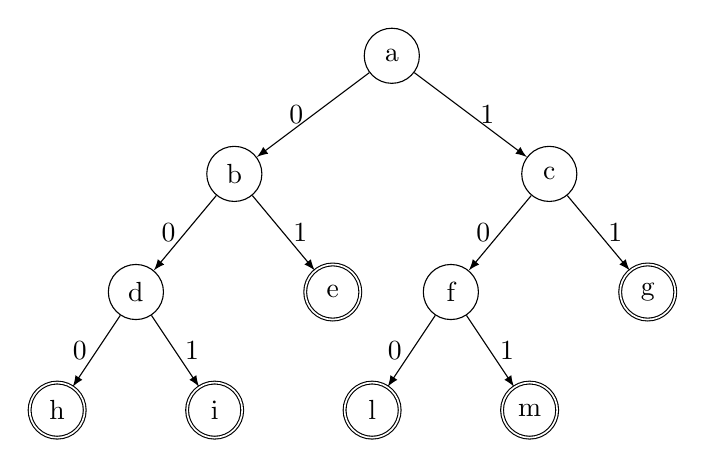
\begin{tikzpicture}[
            level distance=1.5cm,
            sibling distance=3cm,
            state/.style={circle, draw, minimum size=7mm},
            accepting/.style={circle, draw, double, minimum size=7mm},
            edge from parent/.style={draw, -latex},
            level 1/.style={sibling distance=4cm},
            level 2/.style={sibling distance=2.5cm},
            level 3/.style={sibling distance=2cm}
            ]
        
        \node[state] (a) {a}
            child {node[state] (b) {b} 
            child {node[state] (d) {d}
                child {node[accepting] (h) {h}}
                child {node[accepting] (i) {i}}
            }
            child {node[accepting] (e) {e}}
            }
            child {node[state] (c) {c}
            child {node[state] (f) {f}
                child {node[accepting] (l) {l}}
                child {node[accepting] (m) {m}}
            }
            child {node[accepting] (g) {g}}
            };
        
        % Etichette degli archi
        \path (a) -- (b) node[midway, left] {0};
        \path (a) -- (c) node[midway, right] {1};
        \path (b) -- (d) node[midway, left] {0};
        \path (b) -- (e) node[midway, right] {1};
        \path (c) -- (f) node[midway, left] {0};
        \path (c) -- (g) node[midway, right] {1};
        \path (d) -- (h) node[midway, left] {0};
        \path (d) -- (i) node[midway, right] {1};
        \path (f) -- (l) node[midway, left] {0};
        \path (f) -- (m) node[midway, right] {1};
        \end{tikzpicture}
        \caption{Example ADFA to be minimized}
        \label{fig:example_ADFA}
    \end{figure}

    Now, let us apply the minimization algorithm step by step:
    \begin{enumerate}
        \item \textbf{Height Computation:} First, we compute the height of each state. The height is the length of the longest path to a final state. The final states ($e, g, h, i, l, m$) have a height of 0. For the other states, the height is calculated as follows:
        \begin{itemize}
            \item $h(d) = 1 + \max(h(h), h(i)) = 1 + 0 = 1$
            \item $h(f) = 1 + \max(h(l), h(m)) = 1 + 0 = 1$
            \item $h(b) = 1 + \max(h(d), h(e)) = 1 + \max(1, 0) = 2$
            \item $h(c) = 1 + \max(h(f), h(g)) = 1 + \max(1, 0) = 2$
            \item $h(a) = 1 + \max(h(b), h(c)) = 1 + \max(2, 2) = 3$
        \end{itemize}
        This gives us the following partitions based on height:
        \begin{itemize}
            \item $\Pi_0 = \{e, g, h, i, l, m\}$
            \item $\Pi_1 = \{d, f\}$
            \item $\Pi_2 = \{b, c\}$
            \item $\Pi_3 = \{a\}$
        \end{itemize}

        \item \textbf{Processing $\Pi_0$:} All states in $\Pi_0$ are final and have no outgoing transitions, so they are all equivalent. We merge them into a single class, let us call it $D = \{e, g, h, i, l, m\}$. After this step, we have a new state $D$ which is final.

        \item \textbf{Processing $\Pi_1$:} Now we examine the states in $\Pi_1$: $d$ and $f$. We check their transitions:
        \begin{itemize}
            \item State $d$: $\delta(d, 0) = h \in D$ and $\delta(d, 1) = i \in D$.
            \item State $f$: $\delta(f, 0) = l \in D$ and $\delta(f, 1) = m \in D$.
        \end{itemize}
        Since both states transition to the same equivalence class ($D$) for both symbols $0$ and $1$, they are equivalent. We merge them into a new class, $C = \{d, f\}$.

        \item \textbf{Processing $\Pi_2$:} Next, we process the states in $\Pi_2$: $b$ and $c$.
        \begin{itemize}
            \item State $b$: $\delta(b, 0) = d \in C$ and $\delta(b, 1) = e \in D$.
            \item State $c$: $\delta(c, 0) = f \in C$ and $\delta(c, 1) = g \in D$.
        \end{itemize}
        Both states have transitions to class $C$ on symbol $0$ and to class $D$ on symbol $1$. Therefore, $b$ and $c$ are equivalent. We merge them into a new class, $B = \{b, c\}$.

        \item \textbf{Processing $\Pi_3$:} Finally, we process $\Pi_3$, which contains only state $a$. There is nothing to compare it with, so it forms its class, $A = \{a\}$.
    \end{enumerate}

    After applying the algorithm, we obtain the minimized ADFA represented in \cref{fig:example_minimized_ADFA}. Each node of the original ADFA is represented by a node in the minimized ADFA (equivalence classes). The edges represent transitions between these nodes. The root node $A$ is the initial state of the minimized ADFA, while the node $D$ is the final state.
    
    \begin{figure}[H]
        \centering
        \begin{tikzpicture}[->, >=stealth, node distance=3cm, on grid, auto]
            \node[state, initial, initial text=] (A) {A};
            \node[state] (B) [right=of A] {B};
            \node[state] (C) [right=of B] {C};
            \node[state, accepting] (D) [right=of C] {D};
        
            \path (A) edge [bend left] node {0} (B)
                    edge [bend right] node[below] {1} (B)
                (B) edge [bend left] node {0} (C)
                    edge [bend right] node[below] {1} (D)
                (C) edge [bend left] node {0} (D)
                    edge [bend right] node[below] {1} (D);
        \end{tikzpicture}
        \caption{Minimized ADFA}
        \label{fig:example_minimized_ADFA}
    \end{figure}      

    The equivalence classes of the nodes are listed in \cref{tab:equivalence_classes}.
    
    \begin{table}[H]
        \centering
        \begin{tabular}{|c|l|}
            \hline
            \textbf{Class} & \textbf{States} \\
            \hline
            A & $a$ \\
            B & $b, c$ \\
            C & $d, f$ \\
            D & $e, g, h, i, l, m$ \\
            \hline
        \end{tabular}
        \caption{Equivalence classes of the nodes}
        \label{tab:equivalence_classes}
    \end{table}
\end{example}